We used the SEE system call interface to build a model for the POSIX interface.
%
In this section, we describe the key design decisions involved in building the model, and we illustrate the use of the symbolic system call interface.
%
This also serves as an example for building additional models on top of the \cnine symbolic system call interface.

The POSIX model uses shared memory structures to keep track of all system objects (processes, threads, sockets, etc.).
%
The two most important data structures are stream buffers and block buffers, analogous to character and block device types in UNIX.  Stream buffers model half-duplex communication channels: they are generic producer-consumer queues of bytes, with support for event notification to multiple listeners.  Event notifications are used, for instance, by the polling component in the POSIX model.  Block buffers are random-access, fixed-size buffers, whose operations do not block; they are used to implement symbolic files.

The symbolic execution engine maintains only basic information on running processes and threads: identifiers, running status, and parent--child information.
%
However, the POSIX standard mandates additional information, such as open file descriptors and permission flags. This information is stored by the model in auxiliary data structures associated with the currently running threads and processes. The implementations of \codebit{fork()} and \codebit{pthread\_create()} are in charge of initializing these auxiliary data structures and making the appropriate symbolic system calls.

Modeling synchronization routines is simplified by the cooperative scheduling policy:
%
no locks are necessary, and all synchronization can be done using the sleep/notify symbolic system calls, together with reference counters.  Figure~\ref{fig:mutexcode} illustrates the simplicity this engenders in the implementation of pthread mutex lock and unlock.

\begin{figure}
  \centering
  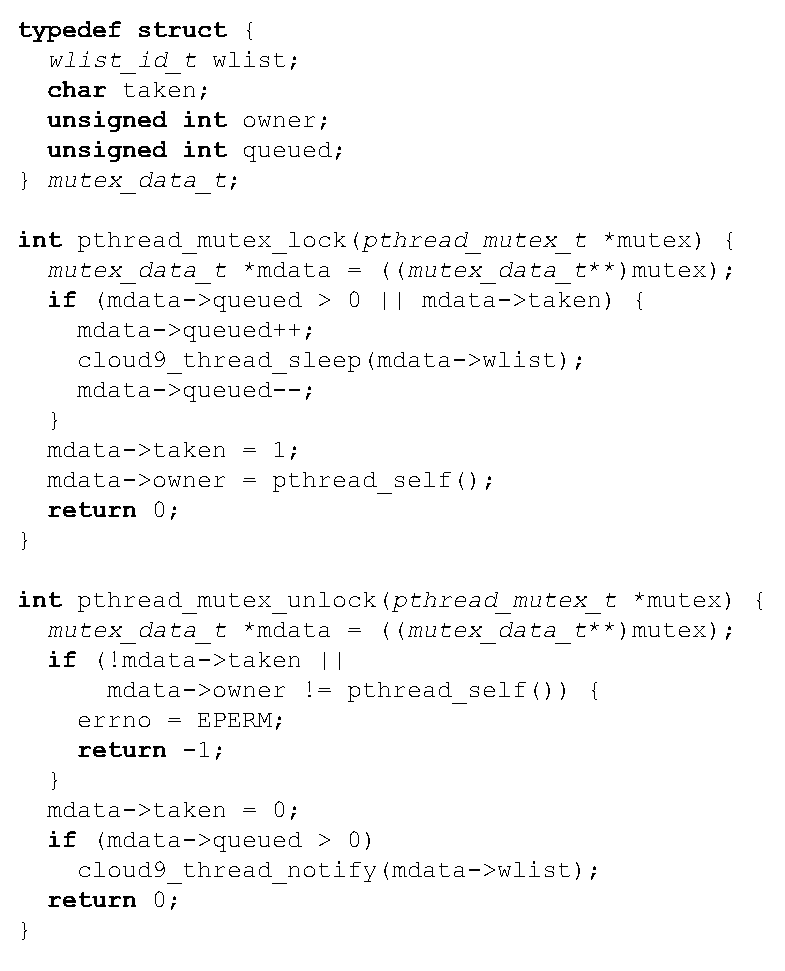
\epsfig{file=cloud9/figures/mutex-model.eps, width=3.2in}
  \caption{Example implementation of pthread mutex operations in \cnine's POSIX environment model.}
  \label{fig:mutexcode}
\end{figure}

\cnine uses most of \klee's file model semantics.
%
In particular, one can either open a symbolic file (its contents comes from a symbolic block buffer), or a concrete file, in which case a concrete file descriptor is associated with the symbolic one, and all operations on the file are forwarded as external calls on the concrete descriptor. 

\begin{figure}
  \centering
  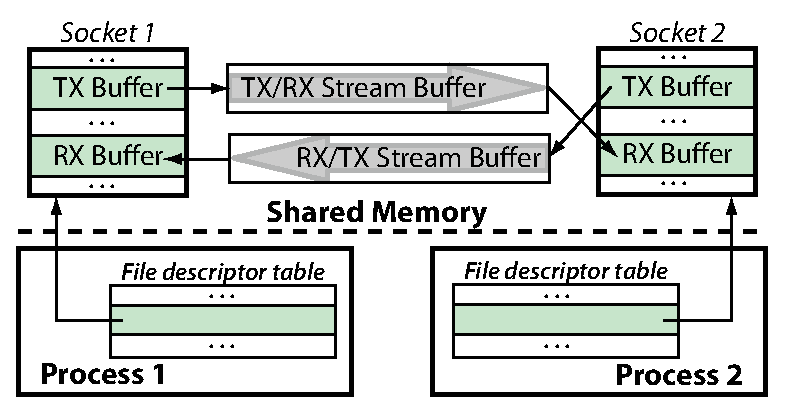
\epsfig{file=cloud9/figures/network-model.eps, width=4.0in}
  \caption{A TCP network connection is modeled in \cnine using TX and RX buffers implemented as stream buffers.}
  \label{fig:networkmodel}
\end{figure}

In addition to file objects, the \cnine POSIX model adds support for networking and pipes.
%
Currently, the TCP and UDP protocols are supported over IP and UNIX network types. Since no actual hardware is involved in the packet transmission, we can collapse the entire networking stack into a simple scheme based on two stream buffers (Figure~\ref{fig:networkmodel}). The network is modeled as a single-IP network with multiple available ports---this configuration is sufficient to connect multiple processes to each other, in order to simulate and test distributed systems. The model also supports pipes through the use of a single stream buffer, similar to sockets.

The \cnine POSIX model supports polling through the \codebit{select()} interface.
%
All the software we tested can be configured to use \codebit{select()}, so it was not necessary to implement other polling mechanisms.  The \codebit{select()} model relies on the event notification support offered by the stream buffers that are used in the implementation of blocking I/O objects (currently sockets and pipes).

The constraint solver used in \cnine operates on bit vectors; as a result, symbolic formulas refer to contiguous areas of memory.
%
In order to reduce the constraint solving overhead, we aim to reduce the amount of intermixing of concrete and symbolic data in the same memory region.  Thus, \cnine's POSIX model segregates concrete from symbolic data by using static arrays for concrete data and linked lists (or other specialized structures) for symbolic data.  We allocate into separate buffers potentially-symbolic data passed by the tested program through the POSIX interface.

In order to enable testing the systems presented in the evaluation section (Section~\ref{sec:eval:targets}), we had to add support for various other components: IPC routines, \codebit{mmap()} calls, time-related functions, etc.
%
Even though laborious, this was mostly an engineering exercise, so we do not discuss it further.

Finally, in some cases, it is practical to have the host OS handle parts of the environment via \emph{external calls}.
%
These are implemented by concretizing the symbolic parameters of a system call before invoking it from symbolically executing code. Unlike \cite{dart,klee,exe}, \cnine allows external calls \emph{only} for stateless or read-only system calls, such as reading a system configuration file from the \codebit{/etc} directory.  This restriction ensures that external concrete calls do not clobber other symbolically executing paths.

%%% Local Variables: 
%%% mode: latex
%%% eval: (visual-line-mode)
%%% fill-column: 1000000
%%% TeX-master: "main"
%%% End:
